\documentclass[11pt]{article}
\usepackage{amsmath,amsthm,amsfonts,amssymb,amscd}
\usepackage{multirow,booktabs}
\usepackage[table]{xcolor}
\usepackage{fullpage}
\usepackage{lastpage}
\usepackage{enumitem}
\usepackage{fancyhdr}
\usepackage{mathrsfs}
\usepackage{wrapfig}
\usepackage{setspace}
\usepackage{calc}
\usepackage{multicol}
\usepackage{cancel}
\usepackage[retainorgcmds]{IEEEtrantools}
\usepackage[margin=3cm]{geometry}
\usepackage{empheq}
\usepackage{framed}
\usepackage[most]{tcolorbox}
\usepackage{xcolor}
\usepackage{graphicx}
\colorlet{shadecolor}{orange!15}
\newlength{\tabcont}
\setlength{\parindent}{0.0in}
\setlength{\parskip}{0.05in}
\parindent 0in
\parskip 12pt
\geometry{margin=1in, headsep=0.25in}
\theoremstyle{definition}
\newtheorem{defn}{Definition}
\newtheorem{reg}{Rule}
\newtheorem{exer}{Exercise}
\newtheorem{note}{Note}
\begin{document}
\title{Chapter 9 Review Notes}
\thispagestyle{empty}
\begin{center}
{\LARGE \bf Homework 2}\\
{\large Guoyuan Liu}\\
Fall 2023, PHYS-467
\end{center}

\section*{Question 2}
Notice $P(G|\{g_i\}, \theta)$ is similar to binomial distribution with the probability of success, or the existence of an edge, as a variable. So we can write
\begin{equation}
    \label{eq: 1}
    P(G|\{g_i\}, \theta) = \prod_{i\neq j}^N p_{g_i,g_j}^{A_{ij}} (1 - p_{g_i , g_j}^{A_{ij}})^{(1-A_{ij})}
\end{equation}
and the assignment of $g_i$ is just
\begin{equation}
    \label{eq: 2}
    P(\{g_i\}|\theta) = \prod_i^N n_{g_i}
\end{equation}
With Bayes' theorem, we have
\begin{align*}
        P(\{g_i\}| G, \theta) = \frac{P(G|\{g_i\}, \theta) P(\{g_i\}|\theta)}{\sum_{\{g_i\}} P(G|\theta)},
\end{align*}
substitute equation \ref{eq: 1} and \ref{eq: 2} into above, the nominator becomes
\begin{align*}
    P(G|\{g_i\}, \theta) P(\{g_i\}|\theta) &= \prod_{i\neq j}^N p_{g_i,g_j}^{A_{ij}} (1 - p_{g_i , g_j}^{A_{ij}})^{(1-A_{ij})} \prod_i^N n_{g_i}\\
    &= \exp(\sum_{i\neq j}^N [A_{ij}\log (p_{g_i,g_j})+(1-A_{ij}) \log (1 - p_{g_i , g_j}^{A_{ij}})] + \sum_i^N \log(n_{g_i})) \\
    &= \exp(- H(\{g_i\}| G, \theta)).
\end{align*}
Since $\sum_{\{g_i\}} P(\{g_i\}|\theta)$ = 1, the denominator is
\begin{align*}
    \sum_{\{g_i\}} P(G|\theta) = \sum_{\{g_i\}} P(G|\{g_i\},\theta) P(\{g_i\}|\theta) = \sum_{\{g_i\}}\exp(- H(\{g_i\}| G, \theta)).
\end{align*}
Thus, we show that
\begin{equation*}
    \mu(\{g_i\}| G, \theta) = P(\{g_i\}| G, \theta) = \frac{\exp(- H(\{g_i\}| G, \theta))}{\sum_{\{g_i\}}\exp(- H(\{g_i\}| G, \theta))}
\end{equation*}


\section*{Question 5}
A MCMC simulation of Stochastic Block Model is run with N = 100, q = 2, $n_0 = 0.7, \quad n_1 = 0.3$ and
$$
P = \begin{pmatrix}
    0.4 & 0.1\\
    0.1 & 0.5\\
\end{pmatrix},
$$
the result is shown in figure below. The energy is steadily decreasing as the system reaches equilibrium around 400 steps. The overlap starts from a small value and reaches 1 at equilibrium. The non-zero fraction, essentially the $n_2$ for the case $q=2$, stablizes to 0.3 at equilibrium, which is the ground truth value.
Note the off-diagonal elements of P is chosen to small to tune down the energy contribution from the interaction among different groups. Thus the system is more likely to reach equilibrium. The result of increased edge probability is shown in figure \ref{fig: q5_large_pab}.
\begin{figure}[t]
    \begin{center}
    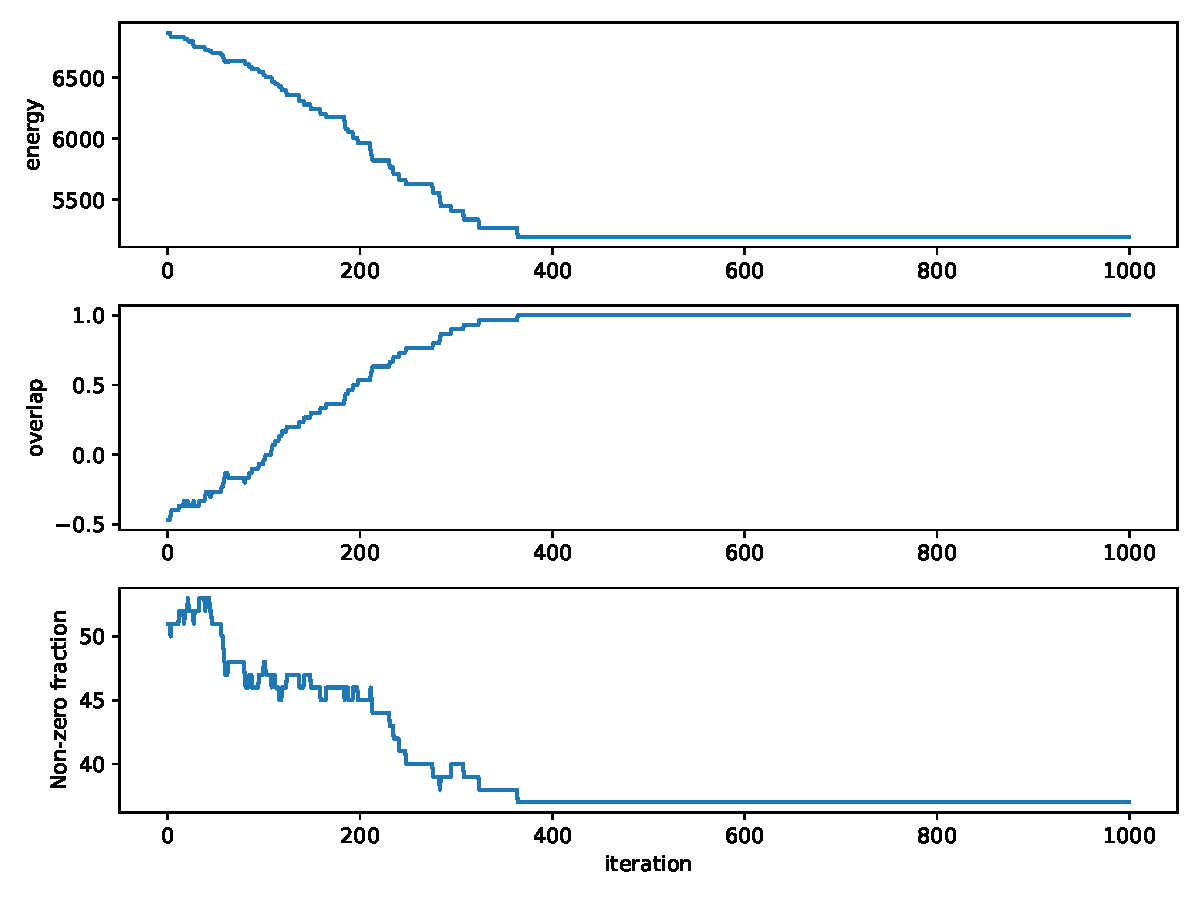
\includegraphics[width=0.8\columnwidth]{./q5_states_small_pab.pdf}
    \caption{MCMC runs for 1000 steps, the evolution of energy, overlap between ground truth and the non-zero fractions is plotted.}
    \end{center}
\end{figure}

\begin{figure}[b]
    \begin{center}
    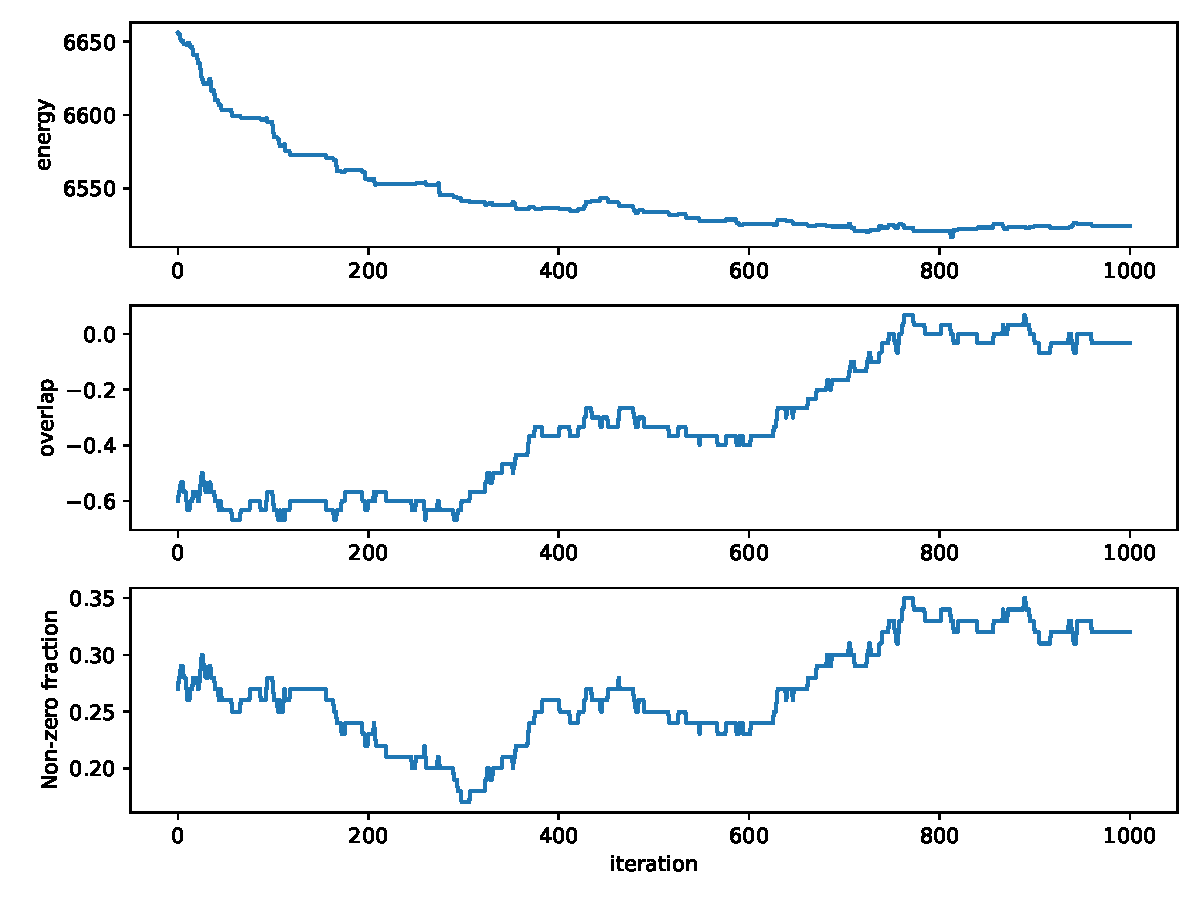
\includegraphics[width=0.8\columnwidth]{./q5_states.pdf}
    \caption{Same MCMC run with increased edge probability. $P_{12} = P_{21} = 0.3$}
    \label{fig: q5_large_pab}
    \end{center}
\end{figure}

\section*{Question 6}
Expected fraction of each group is inferred with Expectation-Maximization algorithm. Initial guess, $\{n_a^0\}_{a=1}^q = \{0.55, 0.45\}$. As the previous question shows the stabilization takes around 400 iterations, for each cycle, MCMC runs for 500 iteration and the stabilized phase is used to calculate the expectation of $\{n_a\}_{a=1}^q$.

The result is shown in figure \ref{fig: q6_runs}. Two reference values are plotted, one is the expectation value used to generate the data, the other is the actual fraction of the sample. They are denoted as expectation and ground truth respectively. The difference between the two is expected to disappear as we increase the simulation size, n.

EM algorithm oscillates around ground truth suggesting more cycle is needed.

\begin{figure}[t]
    \begin{center}
    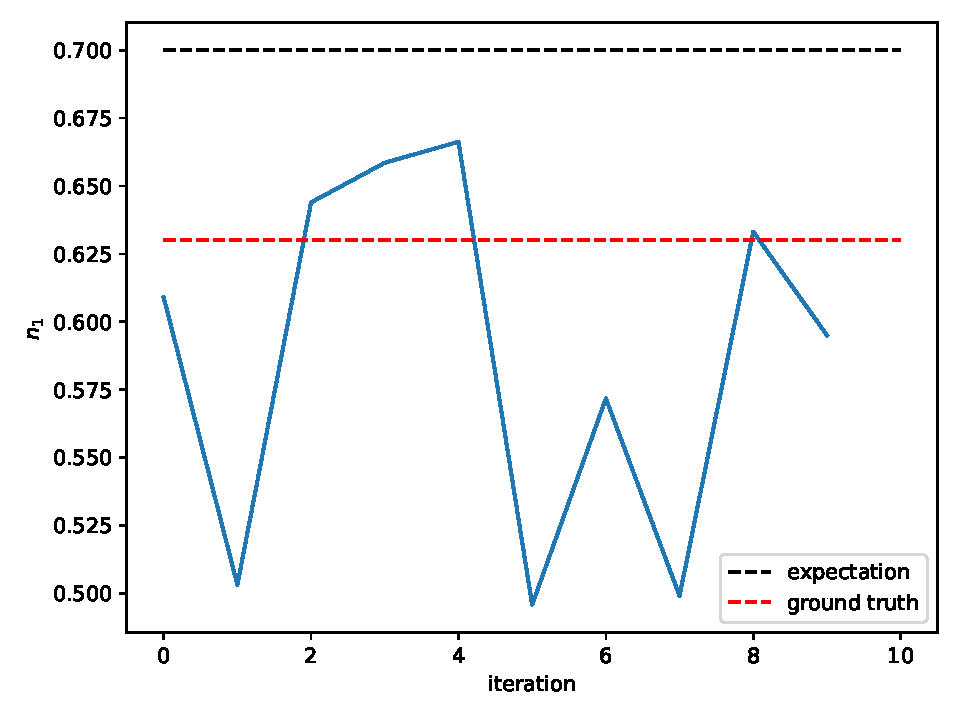
\includegraphics[width=0.8\columnwidth]{./q6_runs_small_pab.pdf}
    \caption{EM runs for 10 cycles, and for each cycle a 500 MCMC run is conducted. The evolution of fraction group 1 is plotted and the ground truth is marked with dash line.}
    \label{fig: q6_runs}
    \end{center}
\end{figure}

\end{document}